\documentclass[11pt,aspectratio=43,ignorenonframetext,t]{beamer}
% Uses fontspec - assumes compiled with LuaLaTeX or similar
% The above \documentclass is for making slides. If making handouts use:
%\documentclass[11pt,a4paper]{article} 
%\usepackage{beamerarticle}
%\setjobnamebeamerversion{main.beamer}

% See https://github.com/CASSON-LAB/uom_beamer_template
% for details on license, further useage information and similar
%%%%%%%%%%%%%%%%%% DOCUMENT SETUP %%%%%%%%%%%%%%%%%%

% Presentation settings
\mode<presentation>{
  \usetheme[framenumber,titleframestart=1]{UoM_alex}
  \usefonttheme{professionalfonts} % using non standard fonts for beamer
  \usefonttheme{serif}             % set font to Arial
  \usepackage{fontspec}
  \setmainfont[Ligatures=TeX]{Arial}
}

% Handout settings
\mode<article>{
  \usepackage{fullpage}                  % use full page
  \usepackage{fontspec}                  % set font to Arial
    \setmainfont[Ligatures=TeX]{Arial}
  \setlength{\parskip}{1.5\baselineskip} % correct beamer line spacings
  \setlength{\parindent}{0cm}
  \usepackage{enumitem}
    \setlist[itemize]{topsep=0pt}
  \definecolor{uomlinkblue}{HTML}{0071BC}
}


% Packages

% Configurando layout para mostrar codigos C++
\usepackage{listings}
\lstset{
  language=HTML,
  basicstyle=\ttfamily\small, 
  keywordstyle=\color{blue}, 
  stringstyle=\color{red}, 
  commentstyle=\color{red}, 
  extendedchars=true, 
  showspaces=false, 
  showstringspaces=false, 
  numbers=left,
  numberstyle=\tiny,
  breaklines=true, 
  backgroundcolor=\color{green!10},
  breakautoindent=true, 
  captionpos=b,
  xleftmargin=0pt,
}

\usepackage{graphicx}  % for graphics files
  \graphicspath{ {./fig/aula3} }
\usepackage{amsmath}   % assumes amsmath package installed
  \allowdisplaybreaks[1] % allow eqnarrays to break across pages
\usepackage{amssymb}   % assumes amsmath package installed 
\usepackage{hyperref} % add hyperlinks to document. Settings are for accessiblity
  \hypersetup{
    colorlinks=true,
    linkcolor=uomlinkblue,
    filecolor=uomlinkblue,      
    urlcolor=uomlinkblue,
	pdflang={en-GB},
}
\usepackage[document]{ragged2e} % left aligned text for accessibility
% experimental - does fundamentally work, if with quite a bit of effort
%\usepackage{axessibility} % LaTeX readable equations for accessibility
%  \tagpdfsetup{tabsorder=structure,uncompress,activate-all,interwordspace=true}
%  \pdfextension catalog{/Lang (en-GB)}
%  \RequirePackage{luacode}
%  \directlua{require("axessibility.lua")}
\usepackage{unicode-math} % unicode maths for accessibility
\usepackage{pdfcomment} % for alt text for accessibility
\usepackage{rotating}  % allow portrait figures and tables
\usepackage{subfigure} % allow matrices of figures
\usepackage{float}     % allows H option on floats to force here placement
\usepackage{multirow}  % allows merging of rows in tables
\usepackage{tabularx}  % allows fixed width tables
\usepackage{ctable}    % modifies \hline for use in table
\usepackage{bm}        % allow bold fonts in equations
\usepackage{pgf}       % allow graphics manipulation
\usepackage{media9}    % allow interactive flash files to be embedded
  \addmediapath{../media}
\usepackage{etoolbox}
  \makeatletter \preto{\@verbatim}{\topsep=0pt \partopsep=0pt} \makeatother  
  
% Custom commands
\newcommand{\matlab}{\emph{\sc{Matlab}}}
\newcommand{\maple}{\emph{\sc{Maple}}}
\newcommand{\simulink}{\emph{\sc{Simulink}}}
\newcommand{\dc}{d.c.}
\newcommand{\ac}{a.c.}
\newcommand{\rms}{RMS}
\newcommand{\wgn}{{\tt wgn}}
\newcommand{\sus}[1]{$^{\mbox{\scriptsize #1}}$}
\newcommand{\sub}[1]{$_{\mbox{\scriptsize #1}}$}
\newcommand{\chap}[1]{Chapter~\ref{#1}}
\newcommand{\sect}[1]{Section~\ref{#1}}
\newcommand{\fig}[1]{Fig.~\ref{#1}}
\newcommand{\tab}[1]{Table~\ref{#1}}
\newcommand{\equ}[1]{(\ref{#1})}
\newcommand{\appx}[1]{Appendix~\ref{#1}}
\newcommand{\degree}{\ensuremath{^\circ}}
\newcommand{\Vrms}{Vrms}
\newcommand{\Vpp}{V\sub{pp}}
\newcommand{\otoprule}{\midrule[\heavyrulewidth]}         
\newcolumntype{Z}{>{\centering\arraybackslash}X}  % tabularx centered columns 
\makeatletter \DeclareRobustCommand{\em}{\@nomath\em \if b\expandafter\@car\f@series\@nil \normalfont \else \bfseries \fi} \makeatother
\newcounter{example_number} % keep track of the example questions



%%%%%%%%%%%%%%%%%% FRONT MATTER %%%%%%%%%%%%%%%%%%
\title{Análise Orientada a objetos}
\subtitle{Aula 3}
\author{Prof. Me. Juliana Costa-Silva}
\begin{document}
%%%%%%%%%%%%%%%%%% TITLE SLIDE %%%%%%%%%%%%%%%%%%
\mode<presentation>{ \frame{\titlepage \label{slide:a}}} 
%\begin{figure}[!ht] 
%\fbox{\includeslide[width=\textwidth]{slide:a}} \end{figure}



%%%%%%%%%%%%%%%%%% NEW SLIDE %%%%%%%%%%%%%%%%%%
\clearpage 
\mode<presentation>{\begin{frame}{Na aula de hoje...}
  \setbeamertemplate{section in toc}[sections numbered]
  \tableofcontents[hideallsubsections]
\end{frame}}
%----------------------------------------------------------------------------
\section{Estruturas de repetição}
\subsection{while}
\mode<presentation>{\begin{frame}{Estrutura de repetição while}
\begin{center}
   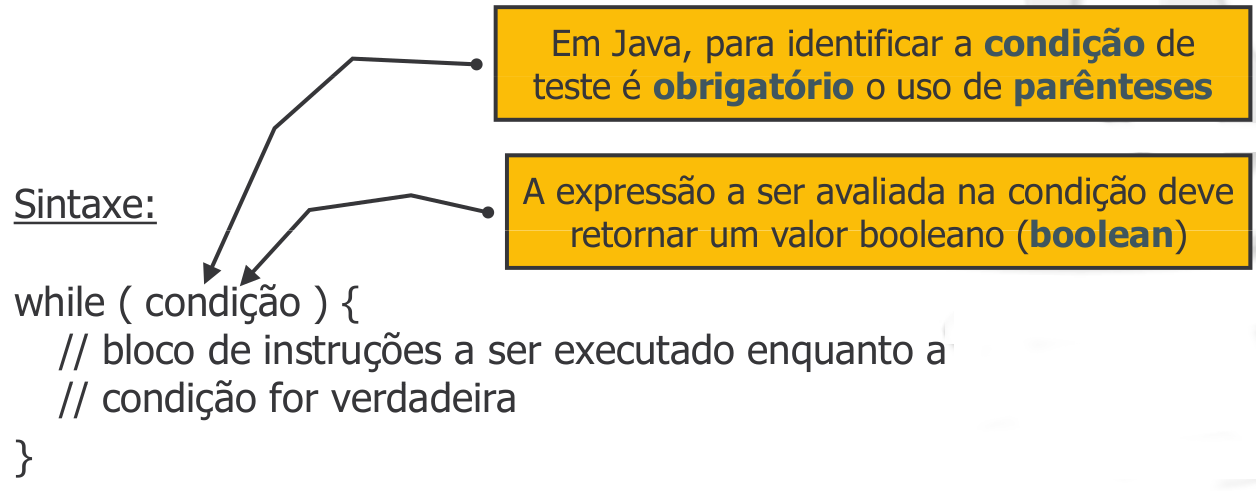
\includegraphics[height=0.45\paperheight]{while.png} \\
 \end{center}
\end{frame}}
%----------------------------------------------------------------------------
\mode<presentation>{\begin{frame}{while (enquanto)}
  \begin{center}
   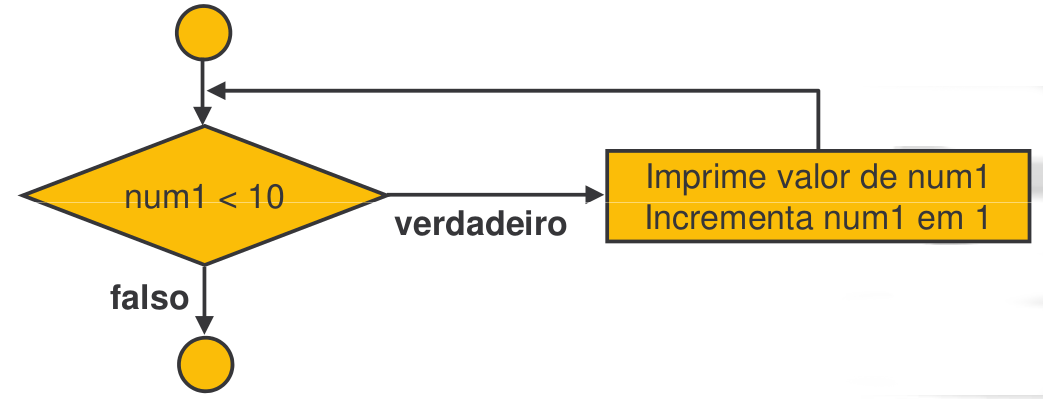
\includegraphics[height=0.25\paperheight]{while_exemplo.png} \\
 \end{center}
  \begin{center} 
   \lstinputlisting[linerange={7-10}]{./cod/Aula4.java}
  \end{center}
\end{frame}}
%----------------------------------------------------------------------------
\mode<presentation>{\begin{frame}{while (enquanto) - Exemplo}
    \begin{center} 
   \lstinputlisting[linerange={11-22}]{./cod/Aula4.java}
  \end{center}
\end{frame}}
%----------------------------------------------------------------------------
\subsection{do/ while}
\mode<presentation>{\begin{frame}{do/ while (faça/ enquanto)}
  Enquanto a condição de teste for verdadeira continua repetindo a execução do 
conjunto definido de instruções. 
\begin{center}
   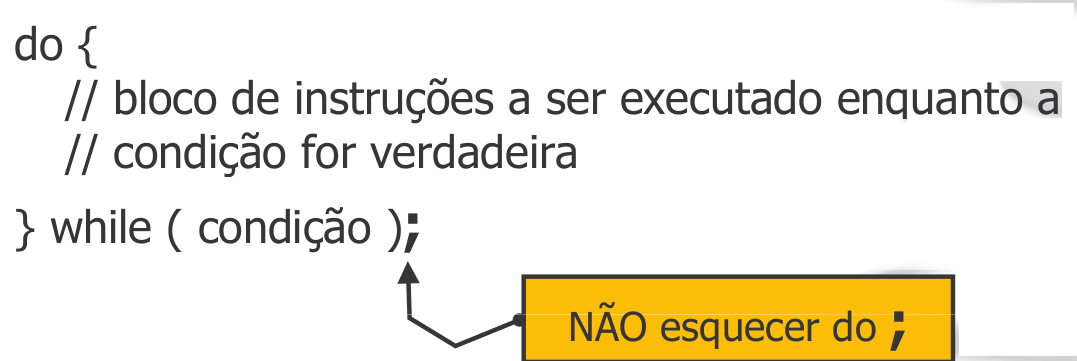
\includegraphics[height=0.25\paperheight]{do_while.png} \\
 \end{center}
 Qual a diferença entre while e do while?\\

A diferença em relação ao while é que o do/while realiza o teste após executar 
pelo menos \textcolor{red}{\textbf{uma vez}} o bloco de instruções.
\end{frame}}
%----------------------------------------------------------------------------
\mode<presentation>{\begin{frame}{do/ while - Exemplo}
  \begin{center}
   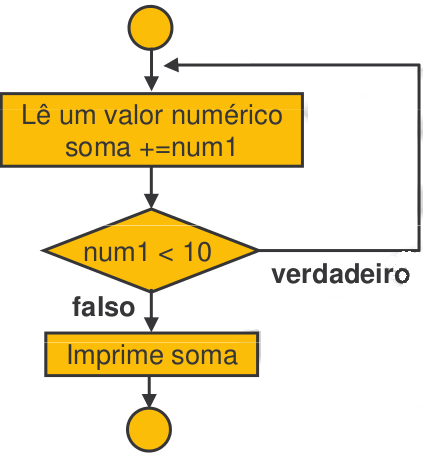
\includegraphics[height=0.3\paperheight]{do_while_exemplo.png} \\
 \end{center}
  \begin{center} 
   \lstinputlisting[linerange={26-31}]{./cod/Aula4.java}
  \end{center}
\end{frame}}
%----------------------------------------------------------------------------
\subsection{for}
\mode<presentation>{\begin{frame}{for}
  Estrutura para execução de um bloco de instruções por repetidas vezes. A 
condição testada para a execução. A condição testada para a execução 
normalmente é baseada em um contador.\\
\begin{center}
   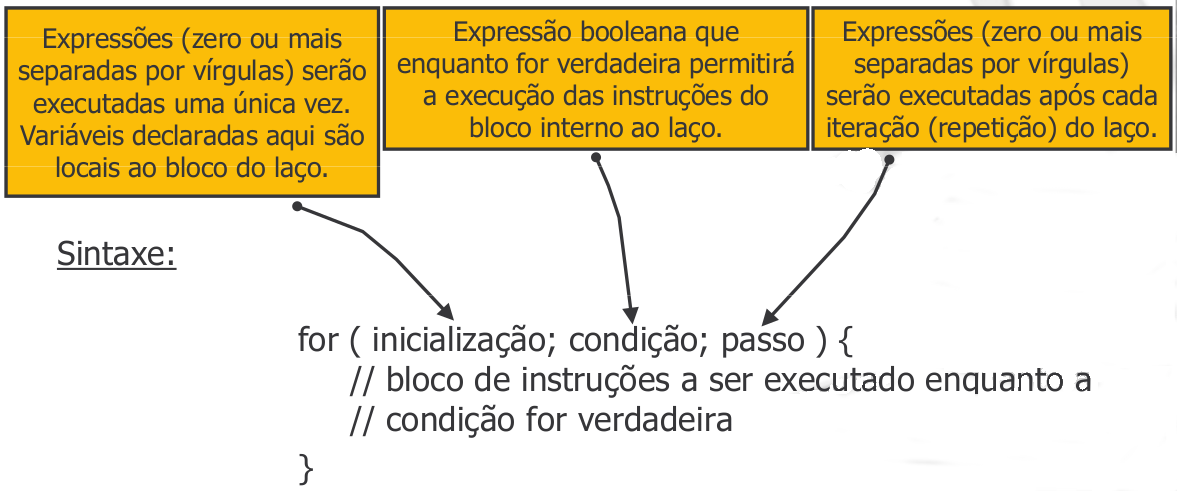
\includegraphics[height=0.45\paperheight]{for.png} \\
 \end{center}
\end{frame}}
%----------------------------------------------------------------------------
\mode<presentation>{\begin{frame}{for - Exemplo}
  
  \begin{center} 
   \lstinputlisting[linerange={34-36}]{./cod/Aula4.java}

   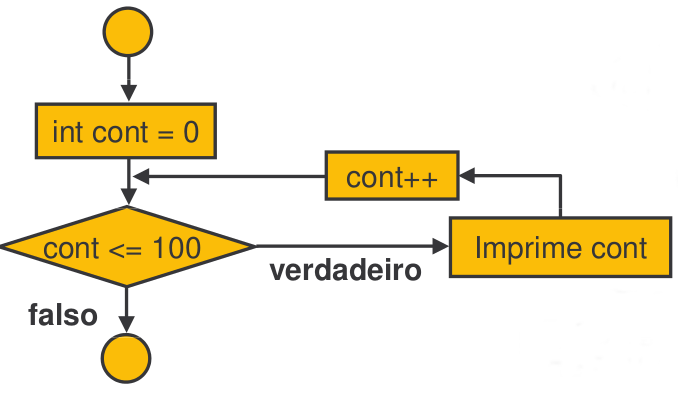
\includegraphics[height=0.4\paperheight]{for_exemplo.png} \\
 \end{center}
\end{frame}}
%----------------------------------------------------------------
\mode<presentation>{\begin{frame}{Exemplos de uso do for}
%   \begin{block}{Exemplos de uso}
    \begin{columns}
      \begin{column}{0.55\textwidth}
	\textcolor{red}{\textbf{1.} }\textbf{for (int i = 1; i $<=$ 100; i++)}\\
      Conta de 1 a 100, de 1 em 1.\\
      \vspace{0.2cm}
      
      \textcolor{red}{\textbf{2.} }\textbf{for (int i = 100; i $>=$ 100; i--)}\\
      Conta de 100 a 1, de 1 em 1.\\
      \vspace{0.2cm}
      
      \textcolor{red}{\textbf{3.} }\textbf{for (int i = 7; i $>=$ 77; i+= 7)}\\
      Conta de 7 a 77, de 7 em 7.\\
      \vspace{0.2cm}
      
      \textcolor{red}{\textbf{4.} }\textbf{for (int i = 20; i $>=$ 20; i -=2 
)}\\
      Conta de 20 a 2, de 2 em 2.\\
      
      \end{column}
      
      \begin{column}{0.55\textwidth}
      
      \textcolor{red}{\textbf{5.} }\textbf{for (int i = 2; i $<=$ 20; i +=3)}\\
      Conta de 2 a 20, de 3 em 3.\\
      
      \textcolor{red}{\textbf{6.} }\textbf{for (; ; )}\\
      Looping infinito.\\
      \vspace{0.2cm}
      
      \textcolor{red}{\textbf{7.} }\textbf{for (int i = 2 ; ; i += 3)}\\
      Looping infinito.\\
      \vspace{0.2cm}
      
      \textcolor{red}{\textbf{8.} }\textbf{for ( ; (i$<$ 10) \&\& j$>$0); )}\\
      Condição composta.\\
      \end{column}
    \end{columns}
%   \end{block}
\end{frame}}
%----------------------------------------------------------------
\section{Desvios em Repetição}
\mode<presentation>{\begin{frame}{Desvios em repetição}
   
  \begin{center} 
   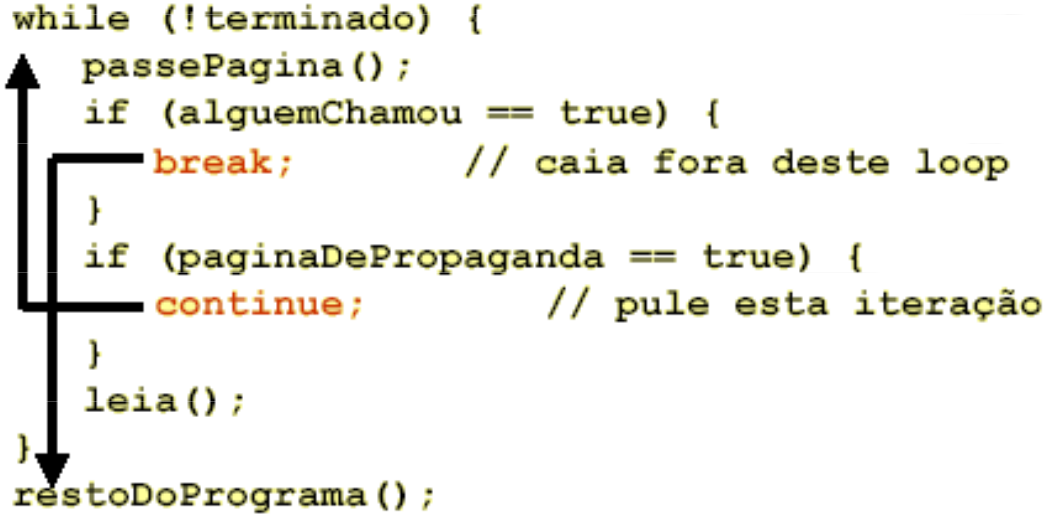
\includegraphics[height=0.6\paperheight]{break_continue.png} \\
 \end{center}

\end{frame}}
%----------------------------------------------------------------------------
\mode<presentation>{\begin{frame}{Desvios em repetição}
  Comando \textbf{break}\\
   \begin{itemize}
   \item \small{Interrompe a execução de um bloco (\textbf{switch, while, do/ 
       while} e \textbf{for}).}
  \end{itemize}

  \vspace{0.2cm}
  Comando \textbf{continue}\\
   \begin{itemize}
     \item \small{Pula as instruções restantes de um bloco (\textbf{while, do/ 
	 while} e \textbf{for}), e realiza a próxima iteração do laço.}
  \end{itemize}

  \begin{block}{\textbf{ATENÇÃO!!}}
  \small{Após o desvio, pelo comando \textcolor{red}{\textbf{continue}}, nas 
estruturas while e do/while, é realizado o teste da condição de repetição.\\
Na estrutura \textbf{for} são executadas as ações de incremento/ decrementoe só 
depois realizado o teste da condição de repetição.}
\end{block}

\end{frame}}
%----------------------------------------------------------------------------
\mode<presentation>{\begin{frame}{Exemplo \textbf{break}}
 \begin{center} 
   \small{
     \lstinputlisting[linerange={40-53}]{./cod/Aula4.java}}
 \end{center}
\end{frame}}
%----------------------------------------------------------------------------
\mode<presentation>{\begin{frame}{Exemplo \textbf{continue}}
 \begin{center} 
   \small{
   \lstinputlisting[linerange={57-67}]{./cod/Aula4.java}
 }
 \end{center}
\end{frame}}
%----------------------------------------------------------------------------
\mode<presentation>{\begin{frame}{Exemplo \textbf{continue} 2}
 \begin{center} 
   \small{
   \lstinputlisting[linerange={71-79}]{./cod/Aula4.java}
 }
 \end{center}
\end{frame}}
%----------------------------------------------------------------
\mode<presentation>{\begin{frame}{Classes Wrappers}
  Java possui algumas classes para auxiliar a utilização de Tipos Primitivos. 
  Estas classes são chamadas de \textcolor{red}{Wrappers}.
  \begin{itemize}
   \item java.lang.Boolean;
   \item java.lang.Character;
   \item java.lang.Byte;
   \item java.lang.Integer;
   \item java.lang.Long;
   \item java.lang.Float;
   \item java.lang.Double;
  \end{itemize}

\end{frame}}
%----------------------------------------------------------------
\mode<presentation>{\begin{frame}{Classes Wrappers}
   Cada uma dessas classes trabalha com o tipo de dados que o seu nome indica;\\
   Todos os métodos são do tipo \textcolor{red}{static} (de classe), ou seja, é 
possível chamá-los sem a necessidade de se criar um objeto de tipo da classe.
\end{frame}}
%----------------------------------------------------------------------------
\mode<presentation>{\begin{frame}{A classe Boolean}
  A classe Boolean provê métodos para a manipulação de tipos primitivos boolean.
\begin{center} 
   \small{
     \lstinputlisting[linerange={4-6}]{./cod/Aula5.java}}
 \end{center}

  \begin{block}{\textbf{valueOf}}
  Converte a String em true ou false caso ela sejam um desses textos, 
independente de maiúsculas e minúsculas.
\end{block}

\end{frame}}
%----------------------------------------------------------------------------
\mode<presentation>{\begin{frame}{Byte, Short, Integer e Long}
  As classes Byte, Short, Integer e Long oferecem maior praticidade na 
manipulação de tipos primitivos inteiros (byte, short, int e long).
 \begin{center} 
   \small{
     \lstinputlisting[linerange={12-15}]{./cod/Aula5.java}}
 \end{center}
\end{frame}}
%----------------------------------------------------------------------------
\mode<presentation>{\begin{frame}{Conversão String $->$ outros tipos de dados}
 \begin{center} 
   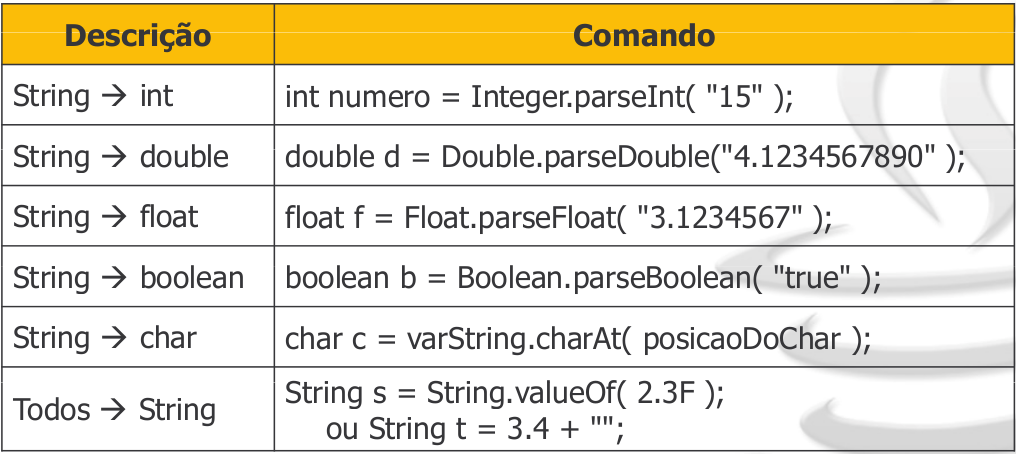
\includegraphics[height=0.45\paperheight]{conversao_string.png} \\
 \end{center}
\end{frame}}
%----------------------------------------------------------------------------
\section{Arrays}
\mode<presentation>{\begin{frame}{Array}
 \begin{center} 
   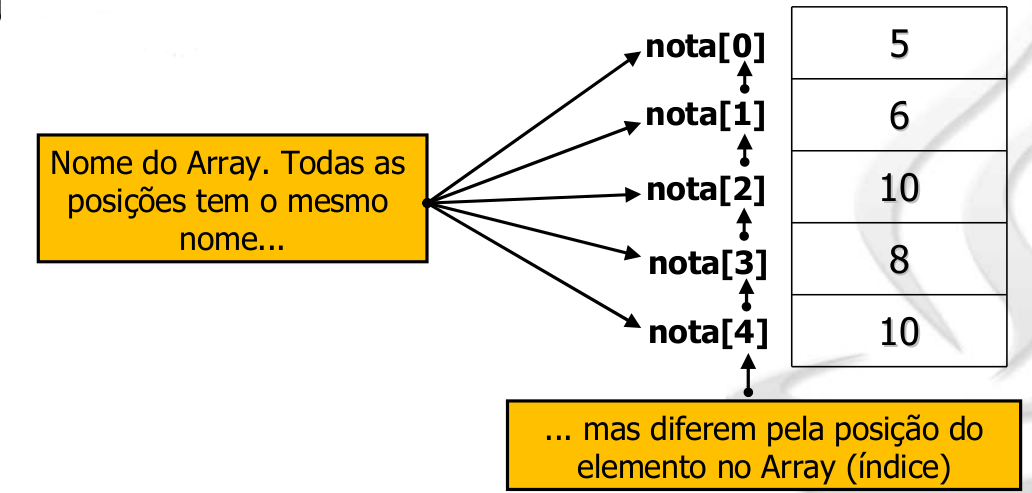
\includegraphics[height=0.4\paperheight]{array.png} \\
   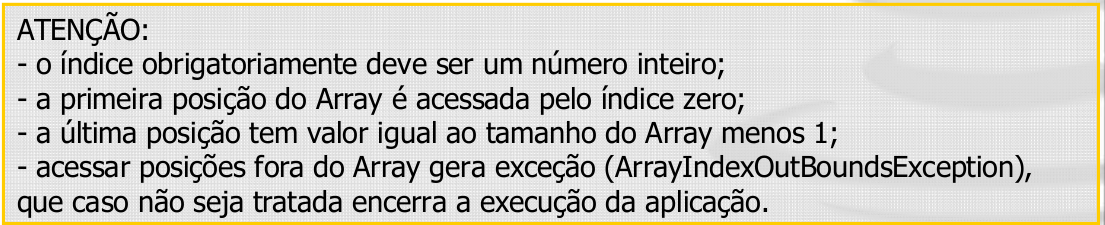
\includegraphics[height=0.2\paperheight]{array_detalhes.png} \\
 \end{center}

\end{frame}}
%----------------------------------------------------------------------
\mode<presentation>{\begin{frame}{Array}
  Para se utilizar um Array é necessário realizar os seguintes passos:
  \begin{itemize}
   \item Declarar a variável do tipo Array
   \item Instanciar o objeto Array (alocar memória)
   \item Inicializar os valores do objeto Array
  \end{itemize}

\end{frame}}
%----------------------------------------------------------------------
\mode<presentation>{\begin{frame}{Declaração de um Array}
  É possíve construir Arrays a partir de um tipo primitivo, ou através de uma 
variável de instância, para referenciar objetos de uma classe.
\begin{center} 
   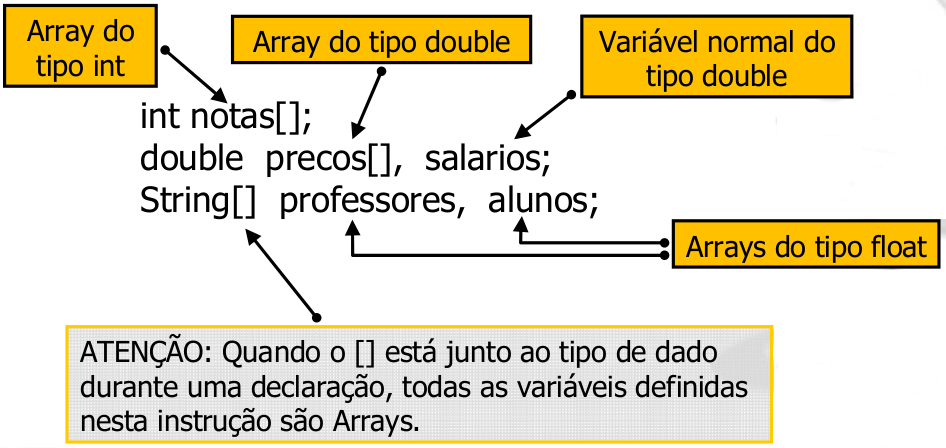
\includegraphics[height=0.4\paperheight]{array_declara.png} \\
 \end{center}

\end{frame}}
%----------------------------------------------------------------------
\mode<presentation>{\begin{frame}{Instanciação de um Array}
  A instanciação do novo array é realizada através do operador 
  \textcolor{red}{new}, como acontece com todos os objetos em Java.
\begin{center} 
   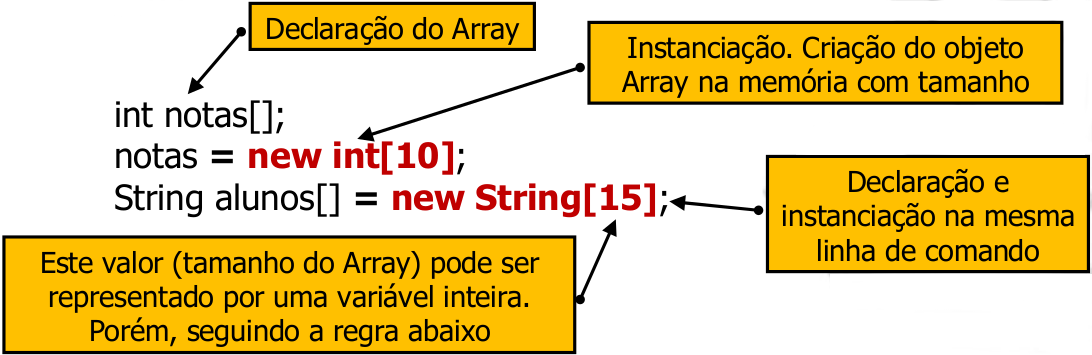
\includegraphics[height=0.35\paperheight]{array_instancia.png} \\
 \end{center}
\end{frame}}
%----------------------------------------------------------------------
\mode<presentation>{\begin{frame}{Inicialização de um Array}
  \small{Após a alocação de um Array todas as sua posiçõe recebem 
    \textbf{implicitamente} um valor padrão nulo.}\\
  \textcolor{purple}{\textbf{Tipos primitivos}}
  \begin{itemize}
    \item \textcolor{red}{byte, short, int} recebem 0 (zero)
    \item \textcolor{red}{long} recebe 0L
    \item \textcolor{red}{float} recebe 0.0F
    \item \textcolor{red}{double} recebe 0.0
    \item \textcolor{red}{char} recebe '$\setminus u0000$'
  \end{itemize}

  \textcolor{purple}{\textbf{Tipos construídos}}
  \begin{itemize}
    \item As variáveis de referência a objetos recebem \textcolor{red}{null}.
  \end{itemize}
  
\end{frame}}
%----------------------------------------------------------------------
\mode<presentation>{\begin{frame}{Inicialização de valores de um Array}
  Após a instanciação de um objeto Array atribuir valores as suas posições 
utilizando-se o índice de acesso a posição.
\begin{center} 
   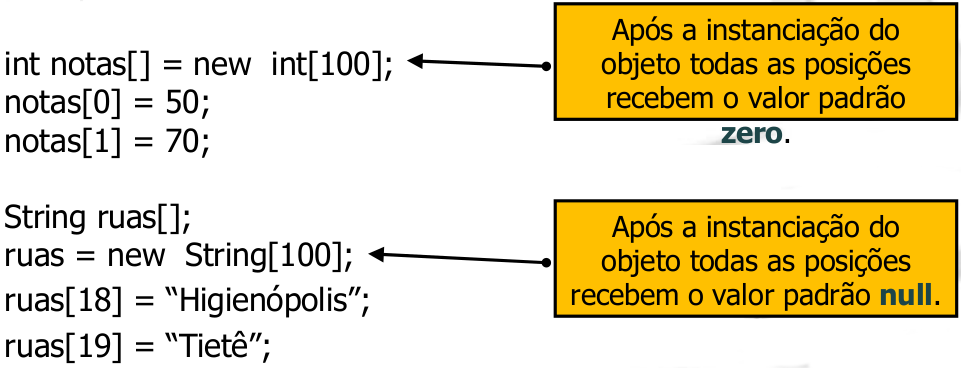
\includegraphics[height=0.4\paperheight]{array_inicia.png} \\
 \end{center}
\end{frame}}
%----------------------------------------------------------------------
\mode<presentation>{\begin{frame}{Inicialização de valores de um Array}
  Após a instanciação de um objeto Array atribuir valores as suas posições 
utilizando-se o índice de acesso a posição.
\begin{center} 
   \small{
     \lstinputlisting[linerange={20-22}]{./cod/Aula5.java}}
 \end{center}
 
\end{frame}}
%----------------------------------------------------------------------
\mode<presentation>{\begin{frame}{Array}
  Utilizando a propriedade de tamanho do Array
\begin{center} 
   \small{
     \lstinputlisting[linerange={25-28}]{./cod/Aula5.java}}
 \end{center}
 Para receber o tamanho de um array, utiliza a propriedade 
  \textcolor{red}{length} do tipo int, que representa a quantidade de elementos 
de um array.
\end{frame}}

%----------------------------------------------------------------------------
\section{Arrays Multidimensionais}
\mode<presentation>{\begin{frame}{Arrays Multidimensionais}
  É possível em Java criar vetores com mais de uma dimensão (arrays 
Multidimensionais).
  \begin{itemize}
    \item Arrays com \textcolor{red}{uma dimensão} são simplesmente chamados de 
vetores.
    \item Arrays com \textcolor{red}{duas dimensões} ou arrays 
   bidimensionais, normalmente são chamados de \textcolor{red}{matrizes} e 
representam uma tabela de valores.
 \item Para arrays com \textcolor{red}{N dimensões} são necessários N 
índices para localizar um elemento, necessitando especificar um índice para 
cada dimensão definida.
  \end{itemize}
\end{frame}}
%----------------------------------------------------------------------------
\mode<presentation>{\begin{frame}{Arrays}{Multidimensionais}
Para os Arrays multidimensionais são válidas as mesmas regras dos Arrays 
unidimensionais
\begin{itemize}
 \item 3 passos (declaração / instanciação / inicialização);
  \item Quando instanciado, todas suas posições recebem valores nulos;
  \item Depois de instanciado é imutável (não altera tamanho).
\end{itemize}

\end{frame}}
%--------------------------------------------e--------------------------------
\mode<presentation>{\begin{frame}{Declaração}{Exemplos}
 \begin{center} 
  Declaração:\\ 
   \small{\lstinputlisting[linerange={3-4}]{./cod/Aula6.java}}
  
   Instanciação:\\ 
  \small{\lstinputlisting[linerange={5-6}]{./cod/Aula6.java}}
  
  Declaração e Instanciação (tudo junto):\\
   \small{\lstinputlisting[linerange={7-8}]{./cod/Aula6.java}}
 \end{center}
\end{frame}}
%--------------------------------------------e--------------------------------
\mode<presentation>{\begin{frame}{Inicialização}{Exemplos}
 \begin{center} 
  Inicialização:\\ 
   
\small{\lstinputlisting[linerange={9-12}]{./cod/Aula6.java}}
  
  Declaração e Instanciação e Inicialização:\\
\small{\lstinputlisting[linerange={13-18}]{./cod/Aula6.java}}
 \end{center}
\end{frame}}
%----------------------------------------------------------------------------
\section{Propriedades}
\mode<presentation>{\begin{frame}{Propriedades}{Array Multidimensional}
  Todo Array multidimensional também possui uma propriedade chamada
\textcolor{red}{length} do tipo \textbf{int}, para cada uma das dimensões que
possui.\\

\textbf{Exemplo:}\\
\begin{center} 
   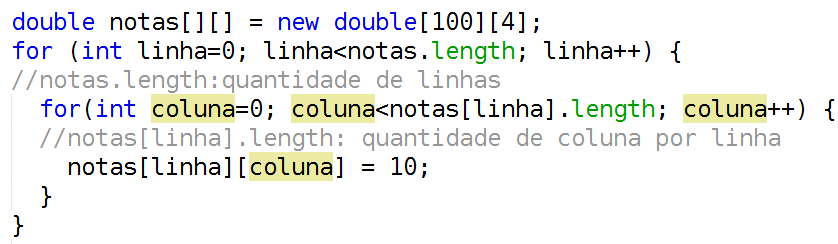
\includegraphics[height=0.35\paperheight]{length_matriz.png} \\
 \end{center}
\end{frame}}

%---------------------------------------------------------------------
\section{Manipulação de Strings}
\mode<presentation>{\begin{frame}{Strings}
 \begin{itemize}
  \item Em Java o tipo \textbf{String não é um tipo primitivo} e simum tipo 
construído, ou seja, \textbf{é uma classe} que encapsula o texto (sequência de 
caracteres) e os métodos para manipula-lo.
   \item A classe String faz parte do pacote \textbf{java.lang} e não 
precisa ser importada explicitamente.
   \item A classe String integra a API básica do Java, por ser uma classe 
de uso fundamental na criação de programas.
 \end{itemize}

\end{frame}}

%---------------------------------------------------------------------
\mode<presentation>{\begin{frame}{Strings}
 \begin{itemize}
  \item É possível criar objetos da classe String atribuindo diretamente uma 
constantes String a uma variável de referência do tipo String.
   \item Outra opção é chamar o construtor da classe String passando a 
constante String como parâmetro.
 \end{itemize}
 
 Opção 1:\\
 \small{\lstinputlisting[linerange={29-29}]{./cod/Aula6.java}}
 Opção 2:\\
 \small{\lstinputlisting[linerange={30-30}]{./cod/Aula6.java}}

\end{frame}}
%---------------------------------------------------------------------
\mode<presentation>{\begin{frame}{Strings}{Tamanho}
É possível identificar quantos caracteres estão armazenados num objeto 
  do tipo String acessando o método \textbf{length()}.
  \vspace{0.5cm}
  \textbf{Exemplo:}
 \small{\lstinputlisting[linerange={32-33}]{./cod/Aula6.java}}
 \end{frame}}
 %---------------------------------------------------------------------
\mode<presentation>{\begin{frame}{Strings}{Comparação}
\textbf{Não é aconselhável }comparar dois objetos String através do operador de 
igualdade (==), pois, as mesmas só terão o mesmo valor caso ambas tenham sido 
% inicializadas com uma constante String idêntica.
%   \vspace{0.5cm}
%   
 \end{frame}}
 %-------------------------------------------------------------------
\mode<presentation>{\begin{frame}{Exemplo}{Comparação de String}
   Receba duas Strings e compare e imprima igual ou diferente.
   
  \begin{center}
    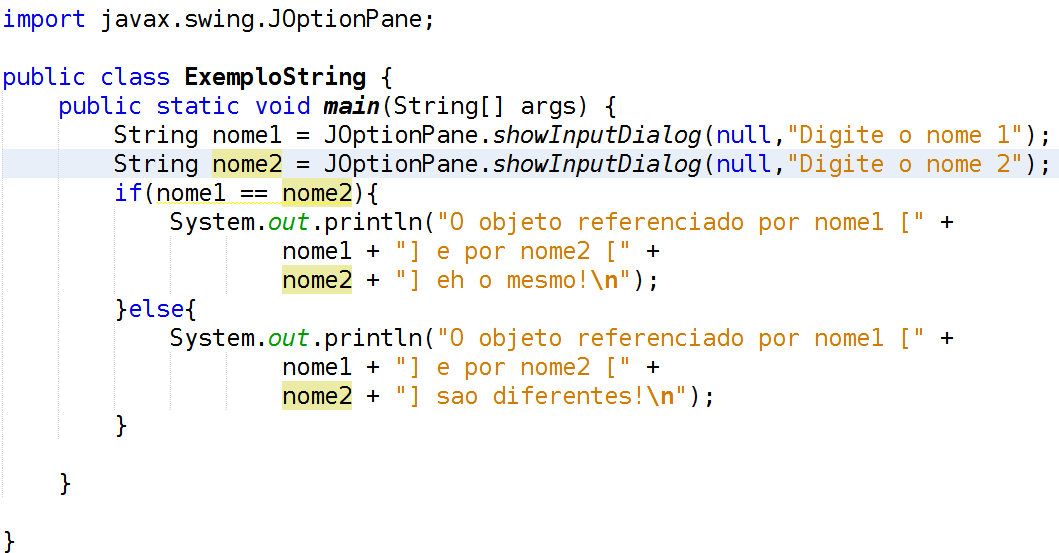
\includegraphics[height=0.6\paperheight]{ExemploString.png} \\
  \end{center}
\end{frame}}
%------------------------------------------------------------------
\mode<presentation>{\begin{frame}{Strings}{Comparação}
  Métodos que comparam Strings\\
  
 Veja o exemplo em ExemploString2.java\\
 
 \vspace{0.5cm}
  Métodos que retiram partes da String\\
  Veja o exemplo em ExemploString3.java\\
\end{frame}}

%----------------------------------------------------------------------
\mode<presentation>{\begin{frame}{Atividades}
  \textbf{1.} Faça um programa em Java que mostre a tabuada de um número 
escolhido pelo usuário (entre 1 e 10). Repita o exercício cm os 3 laços.\\
\vspace{0.5cm}
\textbf{2.} Faça um programa em Java que mostre a tabuada de 1 a 10 em uma 
mesma tela. De 1 a 5 no primeiro bloco e do 6 ao 10 no segundo.
\end{frame}}
%----------------------------------------------------------------------
\mode<presentation>{\begin{frame}{Atividades}
  \textbf{3.} Faça um programa em Java que imprima todos os múltiplos de 3, 
entre 1 e 100.\\
\vspace{0.5cm}
  \textbf{4.} Faça um programa em Java que calcule o fatorial de um número 
pré-definido.\\
\vspace{0.5cm}
  \textbf{5.} Escreva um programa em Java que imprima todos os números múltiplos 
de 5, no intervalo fechado de 1 a 500.

\end{frame}}
%----------------------------------------------------------------------
\section{Atividades}
\mode<presentation>{\begin{frame}{Atividades}
  \textbf{6.} Escreva uma aplicação capaz de receber 10 números (tipo ponto 
flutuante), calcule e imprima: 
\begin{itemize}
 \item Os números digitados; 
 \item A soma dos números; 
 \item A média aritmética entre eles; 
 \item O maior número; 
 \item O menor número.
\end{itemize}
\end{frame}}
%----------------------------------------------------------------------
\mode<presentation>{\begin{frame}{Atividades}
\small
\textbf{7.} Um quadrado mágico é uma matriz quadrada em que a soma das suas linhas é igual a soma das sua colunas e que também é igual a soma da diagonal principal e da diagonal secundária. A matriz abaixo é um exemplo de quadrado mágico, pois a somatória, em todos os casos, é igual a 15.

\begin{center} 
   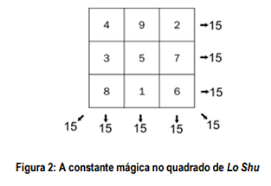
\includegraphics[height=0.2\paperheight]{fig/aula3/quadrado_magico.png} \\
 \end{center}
 Faça um código Java que receba uma dimensão N de uma matriz $A_{nxn}$, seguido dos respectivos valores da matriz (preenchendo a matriz da linha 0 até N, da esquerda para a direta: \textit{coluna 0 até N}), verificar se a matriz é um quadrado mágico (Imprima: “quadrado magico” caso seja e “quadrado NÃO magico” caso não seja).
\end{frame}}
%-----------------------------------------------------
\mode<presentation>{\begin{frame}{Atividades}
  \textbf{8.} Escreva uma aplicação que receba do usuário uma frase no seguinte 
formato N-N-N-...-N-N-N (representando por números inteiros separados por 
hífen), extraia esses números desta frase e crie e alimente um vetor de tamanho 
exato a quantidade de números. De posse desses números, coloque-os em ordem 
decrescente no vetor.
\end{frame}}

%----------------------------------------------------------------------
\mode<presentation>{\begin{frame}{Atividades}
  \textbf{9.} Faça uma aplicação que receba uma frase e retorne o texto invertido.\\
\textbf{10.} Faça uma aplicação que receba o nome completo do usuário, e depois 
troque o seu último sobrenome por Silva. Mostre o resultado na tela.
\end{frame}}
%------------------------------
\section{Leitura recomendada}
\mode<presentation>{\begin{frame}{Leitura complementar}
 Para mais informações sobre JAVA, leia:\\
	\begin{columns}
	\begin{column}{0.5\textwidth}
	 Capítulo 3 a 7:
	 \cite{deitel2017java}
	\end{column}
	\begin{column}{0.4\textwidth}
	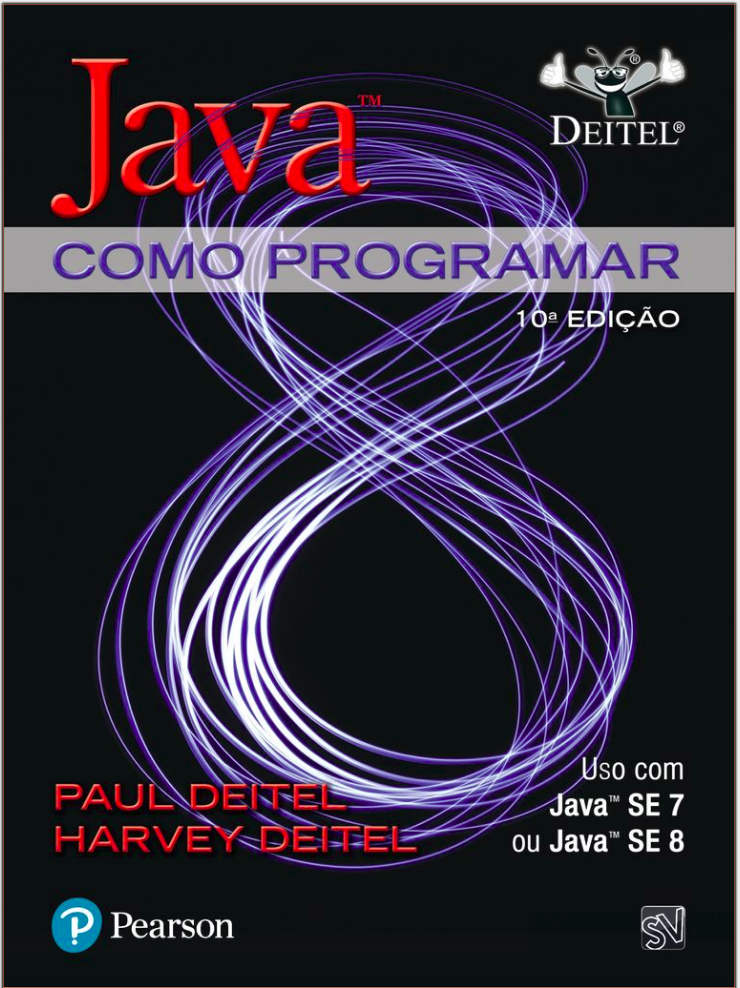
\includegraphics[height=0.6\paperheight]{fig/aula1/deitel2017java.png} 
	\end{column}
	\end{columns}
	%\textcolor{red}{DISPONÍVEL NA BIBLIOTECA VIRTUAL}
\end{frame}}

 %----------------------------------------------------------------------------
 
 \mode<presentation>{\begin{frame}{Referências}%[allowframebreaks]
 \small
 \begin{center}
 	\bibliographystyle{apalike}
	 \bibliography{ref_aula_progI}
 \end{center}
 \end{frame}}

\begin{figure}[!ht] \fbox{\includeslide[width=\textwidth]{slide:z}} \end{figure}
Text for notes goes here. 
\begin{itemize}
  \item List 1. 
  \item List 2. 
\end{itemize}


%%%%%%%%%%%%%%%%%% END MATTER %%%%%%%%%%%%%%%%%%
\end{document}